\section{Results}
\label{sec:results}

\subsection{Size under daily reading}
\label{sec:results-size}

\Cref{fig:paths} shows the mechanism on the generator. On a correct model the log of the e-process drifts down by a small amount on every day without a hit, because the bet loses a little each day, and jumps up on a hit; it rarely approaches the threshold $\log 20$. When the hit rate is three or four times the
nominal the jumps outweigh the drift and the paths cross the threshold, at very different days from stream to stream.

\begin{figure}[htbp]
\centering
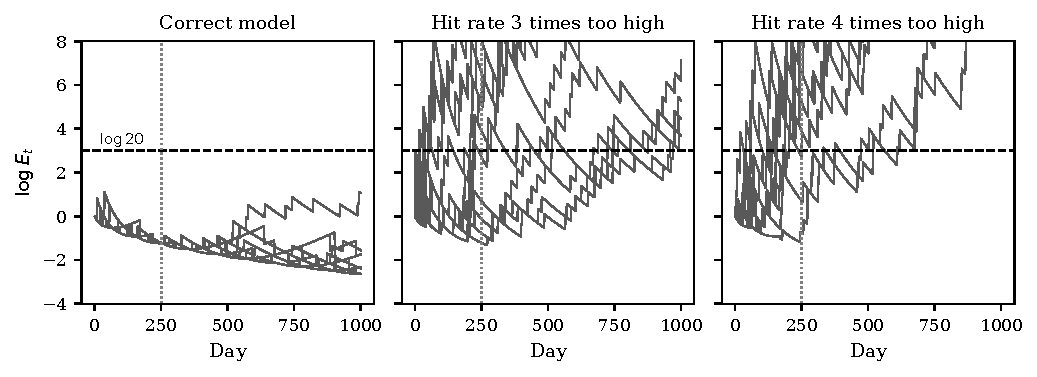
\includegraphics[width=\textwidth]{paths}
\caption{Twelve sample paths of $\log E_t$ of the rate e-process on streams of 1,000 days at a VaR level of 1\,\%: a correct model (left), a hit rate three times the nominal (middle) and four times (right). The dashed line is the rejection threshold $\log 20$ and the dotted line marks day 250, the first day a rule on the last 250 days can speak.}
\label{fig:paths}
\end{figure}

\Cref{tab:main-results} gives the size of every rule when it is read every day over 1,000 days. The rate e-process rejects a correct model in \nNullSizeE\,\% of the \nReps\ series (95\,\% interval \nNullSizeELo\ to \nNullSizeEHi\,\%) and the upper-side variant in \nNullSizeEUp\,\%, both under the acceptance bound of \nBound\,\%; the battery of the rate and clustering monitors in
\nNullSizeBattery\,\% and the clustering monitor alone in \nNullSizeCluster\,\%. The single-alternative likelihood ratio, which has a larger size because it is not spread over alternatives, is at \nNullSizeSprt\,\%, still under 5\,\%. The published e-backtest and the uniform-prior Bayes factor are at \nNullSizeWwz\ and \nNullSizeBeta\,\%. The proposed monitors are conservative, as a mixture
of martingales that starts at one and moves little on correct data should be: the observed size is well below the 5\,\% that \cref{prop:validity} allows. By contrast, the Kupiec test on the last 250 days rejects a correct model in \nNullSizeKupTrail\,\% of the series, the same test on all days so far in \nNullSizeKupCum\,\%, the traffic light leaves its green zone in \nNullSizeLight\,\%,
and the independence test on the last 250 days in \nNullSizeIndep\,\%. The Sidak-corrected Kupiec test controls size at the cost of power (\nNullSizeKupSidak\,\%), and the Kupiec test and the CUSUM with simulated thresholds are at \nNullSizeKupCal\ and \nNullSizeCusum\,\%, at the calibrated size, which the 20,000 calibration streams reproduce to within the
Monte Carlo error of $2{,}000$ streams (a standard error of about 0.5 points).

\begin{table*}[htbp]
\centering
\small
\caption{Every rule read every day on 2,000 streams of 1,000 days from the generator of known truth at a VaR level of 1\,\%: size is the share of correct-model streams rejected at some day, power by day 250 the share of streams with a hit rate three (x3) or four (x4) times too high rejected by day 250, and the median day is the median first-rejection day over all streams (the symbol $>$ marks a median beyond the horizon). Brackets are 95\,\% Wilson intervals for shares and 95\,\% bootstrap intervals for medians. The anytime bound for a size of 5\,\% plus three Monte Carlo standard errors is 6.5\,\%.}
\label{tab:main-results}
\resizebox{\linewidth}{!}{%
\begin{tabular}{p{5.6cm}rrrrr}
\toprule
Rule & Size, \% & Power by day 250, \% (x3) & Median day (x3) & Power by day 250, \% (x4) & Median day (x4) \\
\midrule
\relax Rate e-process, two-sided (proposed) & \relax 2.4 [1.8, 3.2] & \relax 48.6 [46.5, 50.8] & \relax 259 [237, 273] & \relax 77.8 [76.0, 79.6] & \relax 130 [125, 134] \\
\relax Rate e-process, upper side (proposed) & \relax 2.5 [1.9, 3.3] & \relax 55.4 [53.2, 57.5] & \relax 232 [221, 240] & \relax 82.5 [80.8, 84.1] & \relax 119 [108, 129] \\
\relax Single alternative, $3\alpha$ (likelihood-ratio e-process) & \relax 3.6 [2.9, 4.5] & \relax 62.5 [60.4, 64.6] & \relax 182 [176, 202] & \relax 86.1 [84.5, 87.5] & \relax 114 [111, 119] \\
\relax Rate and clustering e-processes, averaged (proposed) & \relax 1.2 [0.8, 1.8] & \relax 39.6 [37.5, 41.8] & \relax 320 [301, 332] & \relax 73.0 [71.0, 74.9] & \relax 158 [151, 161] \\
\relax E-backtest of Wang, Wang and Ziegel (2022) & \relax 0.4 [0.2, 0.8] & \relax 22.4 [20.6, 24.3] & \relax 408 [395, 422] & \relax 53.8 [51.6, 55.9] & \relax 237 [231, 246] \\
\relax Uniform-prior Bayes factor & \relax 0.8 [0.5, 1.3] & \relax 29.8 [27.8, 31.8] & \relax 433 [416, 462] & \relax 61.7 [59.5, 63.8] & \relax 200 [192, 206] \\
\relax Kupiec, last 250 days, read daily & \relax 65.7 [63.6, 67.7] & \relax 62.4 [60.2, 64.4] & \relax 250 [250, 250] & \relax 87.1 [85.6, 88.5] & \relax 250 [250, 250] \\
\relax Kupiec, all days so far, read daily & \relax 31.9 [29.9, 34.0] & \relax 79.0 [77.1, 80.7] & \relax 117 [110, 121] & \relax 94.2 [93.0, 95.1] & \relax 68 [66, 70] \\
\relax Basel traffic light, read daily & \relax 58.8 [56.6, 60.9] & \relax 87.0 [85.5, 88.4] & \relax 250 [250, 250] & \relax 97.2 [96.4, 97.8] & \relax 250 [250, 250] \\
\relax Kupiec, all days so far, Sidak level & \relax 0.1 [0.0, 0.3] & \relax 14.8 [13.3, 16.4] & \relax 567 [549, 581] & \relax 41.3 [39.2, 43.5] & \relax 286 [279, 302] \\
\relax Kupiec, all days so far, simulated critical value & \relax 5.3 [4.4, 6.4] & \relax 53.9 [51.8, 56.1] & \relax 239 [230, 245] & \relax 81.5 [79.7, 83.1] & \relax 130 [124, 135] \\
\relax CUSUM against $3\alpha$, simulated threshold & \relax 5.8 [4.9, 6.9] & \relax 46.0 [43.8, 48.2] & \relax 265 [256, 274] & \relax 76.5 [74.6, 78.3] & \relax 165 [159, 172] \\
\bottomrule
\end{tabular}}
\end{table*}


\Cref{fig:size-horizon} follows the share of correct models rejected as the horizon grows to \nHorizonDays\ days. It shows what \cref{tab:main-results} does not: that the size of a repeated rule is not a number but a function of the horizon. The Kupiec test on the last 250 days and the traffic light rise to \nHorizonEndKupTrail\,\% and \nHorizonEndLight\,\% and the Kupiec test on all days so far to \nHorizonEndKupCum\,\%,
as \cref{prop:repeated} says. The e-process reaches \nHorizonEndE\,\%, the e-backtest \nHorizonEndWwz\,\% and the Bayes factor \nHorizonEndBeta\,\% by day \nHorizonDays, under 5\,\% at every horizon, which is the guarantee that holds at any stopping time. The two rules calibrated to a size of 5\,\% over 1,000 days show the limit of a calibration: they are at
\nHorizonThousandKupCal\ and \nHorizonThousandCusum\,\% at day 1,000 and at \nHorizonEndKupCal\ and \nHorizonEndCusum\,\% at day \nHorizonDays. The figure does not say what a monitor detects; that is the subject of the next two subsections.

\begin{figure}[htbp]
\centering
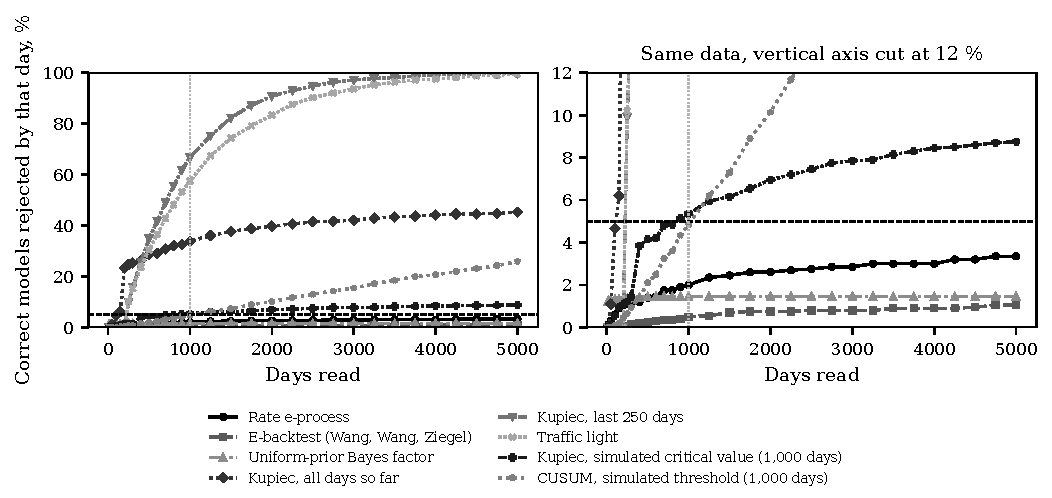
\includegraphics[width=\textwidth]{size-horizon}
\caption{Share of correct VaR models rejected by each rule as a function of the number of days read, from 2,000 streams of 5,000 days at a level of 1\,\% (left, full scale; right, the same curves with the vertical axis cut at 12\,\%). The dashed line is 5\,\% and the dotted line marks the 1,000-day horizon for which two of the rules were calibrated.}
\label{fig:size-horizon}
\end{figure}

\subsection{Detection delay}
\label{sec:results-delay}

\Cref{fig:delay-severity} plots the median first-rejection day and the power by day 250 against the hit-rate multiplier. All rules speed up as the departure grows, and the ranking at each severity is stable. At a hit rate four times the nominal the median day is \nMedFourE\ for the two-sided rate e-process (interval \nMedFourELo\ to \nMedFourEHi) and \nMedFourEUp\ for the upper-side
one, against \nMedFourSprt\ for the single alternative that knows the severity, \nMedFourKupCal\ for the Kupiec test with a simulated constant critical value, \nMedFourKupCum\ for the Kupiec test on all days so far (which has no size guarantee), and \nMedFourLight\ for the traffic light and for the Kupiec test on the last 250 days, which cannot speak before day 250. The published e-backtest
needs \nMedFourWwz\ days and the uniform-prior Bayes factor \nMedFourBeta. The mixture is therefore \nGapFourWwz\ days faster than the e-backtest at that severity (\nMedFourE\ against \nMedFourWwz) and \nGapThreeWwz\ days faster at three times the nominal (\nMedThreeE\ against \nMedThreeWwz), and about as fast as a simulation-calibrated boundary at four times the nominal, where the boundary has a size guarantee for 1,000 days only.

\begin{figure}[htbp]
\centering
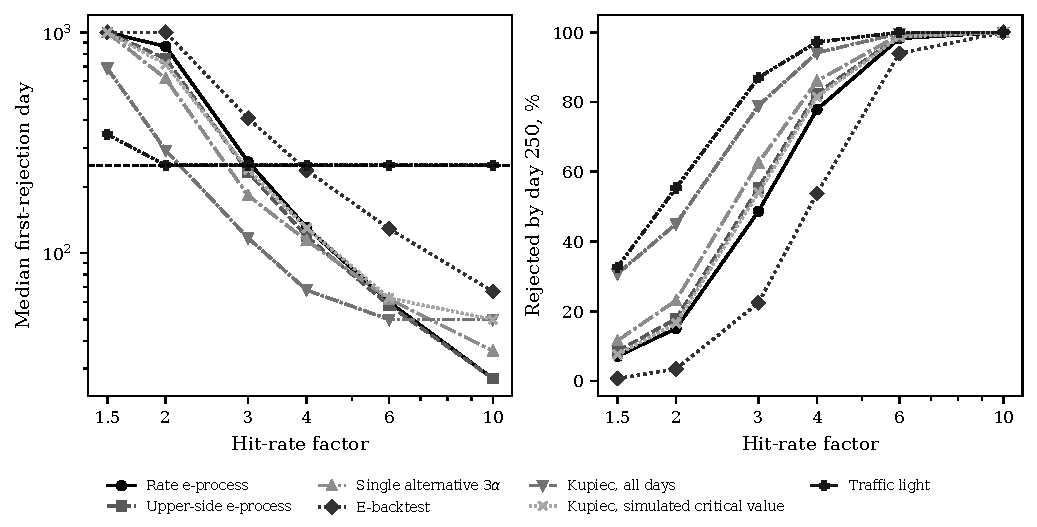
\includegraphics[width=\textwidth]{delay-severity}
\caption{Median first-rejection day (left, logarithmic axes; a point at 1,000 means the median is beyond the horizon) and share of streams rejected by day 250 (right) of the rate e-processes, the single-alternative e-process, the e-backtest and the repeated and calibrated fixed-window rules against the multiplier of the hit rate, 2,000 streams per point; the dashed line is the 250-day window.}
\label{fig:delay-severity}
\end{figure}

At a hit rate three times the nominal, the delay is on the edge of the window. In the main run the two-sided e-process has a median of \nMedThreeE\ days (interval \nMedThreeELo\ to \nMedThreeEHi). The committed document of the product, run with another seed, gives \nCommittedMedThree. \Cref{tab:x3-seeds} settles the question on \nSeedsCount\ independent seeds: the median of the pooled \nSeedsPooledN\ streams is \nSeedsThreeMed\ days (interval \nSeedsThreeMedLo\ to \nSeedsThreeMedHi), the median of single seeds has a mean of \nSeedsThreeSeedMean\ and a standard deviation of \nSeedsThreeSeedSd, and \nSeedsThreeBelow\,\% of the seeds
have a median below 250. The median delay of the two-sided monitor at a hit rate three times the nominal is therefore not distinguishable from the window, and it is not below the traffic light's median of \nSeedsThreeLight. At four times the nominal the pooled median is \nSeedsFourMed\ (interval \nSeedsFourMedLo\ to \nSeedsFourMedHi) and every seed is below 250. The upper-side monitor is below 250 at both severities, \nSeedsUpThreeMed\ days at three times (interval \nSeedsUpThreeMedLo\ to \nSeedsUpThreeMedHi) and \nSeedsUpFourMed\ at four.

\begin{table*}[htbp]
\centering
\small
\caption{The two-sided and the upper-side rate e-process at a hit rate three and four times too high on 20 independent seed sequences of 2,000 streams (40,000 streams per factor): the median first-rejection day of each seed with its mean and standard deviation, the share of seeds whose median is below the 250-day window, the median of the pooled streams with a bootstrap interval, the traffic-light median, and the power cost, the Kupiec power of one reading at day 250 minus the e-process power by day 250, pooled with its standard error and per seed with its standard deviation.}
\label{tab:x3-seeds}
\resizebox{\linewidth}{!}{%
\begin{tabular}{rrrrrrrr}
\toprule
Monitor, hit-rate factor & Mean of seed medians & SD of seed medians & Seeds with median below 250, \% & Pooled median [95\% CI] & Traffic-light median & Power cost, points ($\pm$ SE) & Per-seed power cost, points ($\pm$ SD) \\
\midrule
\relax Two-sided, 3 & 249.7 & 11.6 & \relax 45 & \relax 251.0 [247, 255] & 250 & \relax 12.4 $\pm$ 0.2 & \relax 12.4 $\pm$ 0.7 \\
\relax Two-sided, 4 & 127.7 & 2.7 & \relax 100 & \relax 128.0 [126, 129] & 250 & \relax 8.5 $\pm$ 0.2 & \relax 8.5 $\pm$ 0.7 \\
\relax Upper side, 3 & 227.8 & 6.7 & \relax 100 & \relax 228.0 [225, 231] & 250 & \relax 6.7 $\pm$ 0.2 & \relax 6.7 $\pm$ 0.7 \\
\relax Upper side, 4 & 110.8 & 4.8 & \relax 100 & \relax 109.0 [108, 110] & 250 & \relax 4.6 $\pm$ 0.1 & \relax 4.6 $\pm$ 0.6 \\
\bottomrule
\end{tabular}}
\end{table*}


The reading of the delay needs one caution, which the traffic light makes concrete. Its median of 250 is its first possible day: at three times the nominal it has flagged \nByThreeLight\,\% of the streams by day 250, and the e-process only \nByThreeE\,\%. A median below the window is a statement about the half of the streams detected earliest, not about the share detected by the end of the window.

\subsection{Power by day 250 and its cost}
\label{sec:results-power}

The power of the monitors by day 250 is the cost side of the guarantee. At a hit rate three times the nominal, the two-sided e-process rejects \nByThreeE\,\% of the streams by day 250 (the upper-side one \nByThreeEUp\,\%) against \nShotThree\,\% for one Kupiec reading at day 250 in the same streams; at four times the nominal, \nByFourE\,\% (\nByFourEUp\,\%) against \nShotFour\,\%.
The pooled power cost of the two-sided monitor is \nSeedsThreeCost\ $\pm$ \nSeedsThreeCostSe\ points at three times the nominal and \nSeedsFourCost\ $\pm$ \nSeedsFourCostSe\ points at four times, and that of the upper-side monitor \nSeedsUpThreeCost\ $\pm$ \nSeedsUpThreeCostSe\ and \nSeedsUpFourCost\ $\pm$ \nSeedsUpFourCostSe\ points (\cref{tab:x3-seeds}). The cost is below 10 points at four times the nominal for both monitors and at three times for the upper-side monitor only.

\Cref{tab:size-matched} and \cref{fig:power-size} put the cost in context. The Kupiec test at 250 days and a level of 1\,\% has an expected count of 2.5, so its two-sided size is \nExactKupSize\,\%, of which only \nExactKupUpperSize\,\% lies in the upper tail that rejects an understated VaR (it rejects from \nExactKupMinCount\ exceptions); the large lower-tail share is the probability of no exception in 250 days. The comparison of the monitor with the upper tail of the Kupiec test is therefore a comparison at a similar size, and
at three times the nominal the upper tail has a power of \nExactThreeKupUp\,\%. The most powerful test of the size the e-process spends by day 250 (\nExactESize\,\%) has a power of \nExactThreeNpE\,\% at three times the nominal: no rule with that spending can exceed it (\cref{prop:power}), and the two-sided e-process attains
\nByThreeE\,\% of the \nExactThreeNpE\,\% possible. The upper-side e-process spends more by day 250 (\nExactEUpSize\,\%), so its own bound is higher, \nExactThreeNpEUp\,\%, and it attains \nByThreeEUp\,\%. The cost of the guarantee is largely the cost of spending size over the later days: the mixture gives up power at day 250 to keep the size at every later day.

\begin{table*}[htbp]
\centering
\small
\caption{Exact power at day 250 and a VaR level of 1\,\% (expected count 2.5): the Kupiec test has a size of 9.5\,\% two-sided, of which 1.37\,\% lies in the upper tail that rejects an understated VaR (it rejects from 7 exceptions); the most powerful test, randomised, at the size 1.15\,\% that the rate e-process spends by day 250 on correct models bounds every test of that size; the last two columns are the measured shares of the e-processes on the generator.}
\label{tab:size-matched}
\resizebox{\linewidth}{!}{%
\begin{tabular}{rrrrrr}
\toprule
Hit-rate factor & Kupiec power, two-sided, \% & Kupiec power, upper tail, \% & Best test at the e-process size, \% & Rate e-process by day 250, \% [95\% CI] & Upper-side e-process by day 250, \% [95\% CI] \\
\midrule
\relax 2 & 24.3 & 23.6 & 21.2 & \relax 15.0 [13.5, 16.6] & \relax 17.8 [16.2, 19.5] \\
\relax 3 & 62.5 & 62.5 & 59.1 & \relax 48.6 [46.5, 50.8] & \relax 55.4 [53.2, 57.5] \\
\relax 4 & 87.5 & 87.5 & 85.5 & \relax 77.8 [76.0, 79.6] & \relax 82.5 [80.8, 84.1] \\
\relax 6 & 99.4 & 99.4 & 99.2 & \relax 98.2 [97.6, 98.7] & \relax 98.8 [98.2, 99.2] \\
\bottomrule
\end{tabular}}
\end{table*}


\begin{figure}[htbp]
\centering
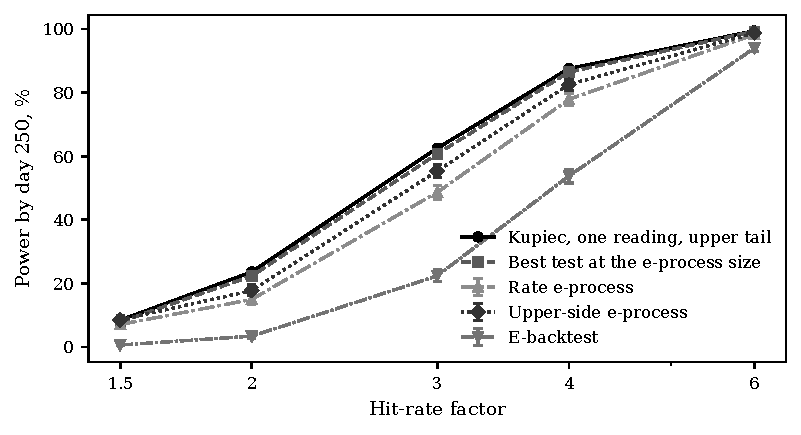
\includegraphics[width=0.85\textwidth]{power-size}
\caption{Power by day 250 against the multiplier of the hit rate at a level of 1\,\%: the exact power of the upper tail of one Kupiec reading, the exact power of the most powerful test at the size the rate e-process spends by day 250, and the measured power of the two-sided and the upper-side rate e-process and of the e-backtest with 95\,\% Wilson intervals, 2,000 streams per point.}
\label{fig:power-size}
\end{figure}

The first-order times of \cref{prop:growth} are compared with the measurements in \cref{tab:theory-delay} and \cref{fig:delay-theory}. The comparison needs the single alternative whose alternative is the true hit rate (the matched bet) at each factor, and the main run measured one single alternative only, the one at three times the nominal level, which is matched at that factor alone. The factors of the table were therefore run again with the matched single alternative on the same streams (an experiment of its own, \texttt{exp\_matched.py}). The matched likelihood ratio reaches the threshold in about \nKlSprtThree\ days at three times the nominal level and \nKlSprtFour\ at four, the mixture of eight alternatives in about \nKlMixThree\ and \nKlMixFour\ days; the measured medians are \nMatchedThreeMed\ and \nMatchedFourMed\ for the matched single alternative and \nMedThreeE\ and \nMedFourE\ for the mixture, all below the first-order times. At every factor from 2 to 10 the matched alternative is faster than the mixture (\nMatchedSixMed\ against \nMedSixE\ days at six times the nominal level and \nMatchedTenMed\ against \nMedTenE\ at ten times), the order of a matched and an unmatched bet that the theory predicts; the single alternative at three times the nominal level, which is matched at that factor only, is slower than the mixture at six and ten times (\nMedSixSprt\ and \nMedTenSprt\ days). The figure shows that the time grows as the inverse of the divergence, so the delay at a hit rate of 1.5 or 2 times the nominal is of the order of years: the mixture has a median of \nMedTwoE\ days at twice the nominal, and at 1.5 times more than half of the streams are not rejected within the 1,000 days (a median \nMedOneFiveE).

\begin{table*}[htbp]
\centering
\small
\caption{The first-order delay of the e-process at a VaR level of 1\,\%: the Kullback-Leibler divergence per day of the true hit rate from the null, in thousandths of a nat, the number of days a log-optimal bet needs to reach the threshold $\log 20$, the same with the penalty $\log K$ of a mixture of $K=8$ alternatives, and the measured median first-rejection days (95\,\% bootstrap intervals) of the single-alternative e-process whose alternative is the true hit rate (matched at every factor) and of the mixture e-process, on the same 2,000 streams. Where the median exceeds the 1,000-day horizon the symbol $>$ is printed.}
\label{tab:theory-delay}
\resizebox{\linewidth}{!}{%
\begin{tabular}{rrrrrr}
\toprule
Hit-rate factor $m$ & $1000\,\mathrm{KL}(m\alpha\|\alpha)$ & Time $\log 20/\mathrm{KL}$ & Time with the mixture penalty & Measured median, matched single alternative & Measured median, mixture \\
\midrule
\relax 1.5 & 1.09 & 2737 & 4636 & \relax $>$1,000 & \relax $>$1,000 \\
\relax 2 & 3.91 & 765 & 1297 & \relax 600 [584, 636] & \relax 862 [830, 920] \\
\relax 3 & 13.16 & 228 & 386 & \relax 182 [177, 203] & \relax 259 [237, 273] \\
\relax 4 & 25.91 & 116 & 196 & \relax 102 [95, 108] & \relax 130 [125, 134] \\
\relax 6 & 58.79 & 51 & 86 & \relax 45 [44, 46] & \relax 60 [58, 62] \\
\relax 10 & 144.48 & 21 & 35 & \relax 17 [16, 18] & \relax 27 [26, 28] \\
\bottomrule
\end{tabular}}
\end{table*}


\begin{figure}[htbp]
\centering
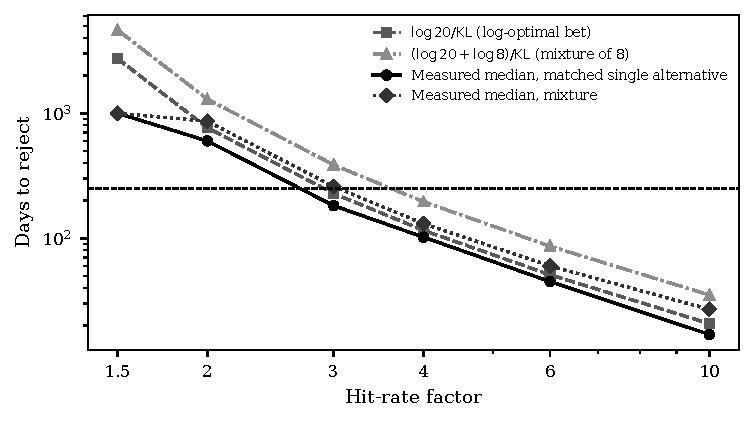
\includegraphics[width=0.8\textwidth]{delay-theory}
\caption{First-order times to reach the threshold $\log 20$ from \cref{prop:growth} (the matched likelihood ratio and the mixture of eight alternatives) and the measured median first-rejection days of the single-alternative and of the mixture e-process against the hit-rate multiplier at a level of 1\,\%; a point at 1,000 means a median beyond the horizon, and the dashed line is the 250-day window.}
\label{fig:delay-theory}
\end{figure}

\subsection{Hit clustering}
\label{sec:results-cluster}

A VaR with the right rate and clustered hits is the second departure. \Cref{tab:clustering} and \cref{fig:clustering} give the share of streams rejected. When hits follow hits with probability $0.4$ (forty times the unconditional rate), the clustering e-process rejects \nCluFourTenthCluster\,\% of the streams within 1,000 days (median \nCluMedFourTenthCluster\ days) and the battery of the two monitors \nCluFourTenthBattery\,\%, while the rate monitor alone rejects \nCluFourTenthE\,\%, more than its size of \nNullSizeE\,\%, because hits that follow hits break the conditional null of the rate monitor even when the rate is right. The Christoffersen test on the last 250 days reads the same departure faster, with a median of \nCluMedFourTenthIndep\ days and \nCluFourTenthIndep\,\% of streams, at a size of \nNullSizeIndep\,\% when it is read every day.
At $q=0.2$ the clustering e-process rejects \nCluTwoTenthCluster\,\% and at $q=0.1$ \nCluOneTenthCluster\,\%, so it is weak against mild clustering, with a median beyond the horizon at $0.1$. The traffic light and the Kupiec test on the last 250 days flag \nCluFourTenthLight\ and \nCluFourTenthKupTrail\,\% of the clustered streams, but they flag \nNullSizeLight\ and \nNullSizeKupTrail\,\% of the correct ones, so their rejection is no evidence of clustering. The Kupiec test with a simulated critical value rejects \nCluFourTenthKupCal\,\% of the clustered streams, because clustering at the right rate changes the count of hits in a window only through its variance.

\begin{table*}[htbp]
\centering
\small
\caption{Share of 1,000-day streams rejected at some day, in percent, when the hit rate is right (1\,\%) and a hit follows a hit with probability $q$ (0.1, 0.2, 0.4), for the proposed clustering monitors, the rate monitor and the fixed-window tests read daily. 2,000 streams per column; brackets are 95\,\% Wilson intervals. The first column is the size of each rule, the other three the power against clustering.}
\label{tab:clustering}
\resizebox{\linewidth}{!}{%
\begin{tabular}{p{6.2cm}rrrr}
\toprule
Rule & \relax Correct model & \relax $q=0.1$ & \relax $q=0.2$ & \relax $q=0.4$ \\
\midrule
\relax Clustering e-process (proposed) & \relax 0.5 [0.3, 0.9] & \relax 25.4 [23.6, 27.4] & \relax 53.8 [51.6, 56.0] & \relax 78.2 [76.3, 80.0] \\
\relax Rate and clustering, averaged (proposed) & \relax 1.2 [0.8, 1.8] & \relax 22.8 [21.0, 24.7] & \relax 51.6 [49.4, 53.8] & \relax 79.8 [78.0, 81.5] \\
\relax Rate e-process (proposed) & \relax 2.4 [1.8, 3.2] & \relax 4.9 [4.0, 5.9] & \relax 6.9 [5.9, 8.1] & \relax 18.6 [16.9, 20.3] \\
\relax Christoffersen independence, last 250 days, read daily & \relax 7.9 [6.8, 9.2] & \relax 57.5 [55.3, 59.6] & \relax 78.6 [76.7, 80.3] & \relax 91.6 [90.3, 92.7] \\
\relax Kupiec, last 250 days, read daily & \relax 65.7 [63.6, 67.7] & \relax 75.4 [73.5, 77.3] & \relax 83.3 [81.6, 84.9] & \relax 94.9 [93.8, 95.8] \\
\relax Basel traffic light, read daily & \relax 58.8 [56.6, 60.9] & \relax 62.8 [60.7, 64.9] & \relax 62.4 [60.3, 64.5] & \relax 68.3 [66.2, 70.3] \\
\relax Kupiec, all days so far, simulated critical value & \relax 5.3 [4.4, 6.4] & \relax 9.0 [7.8, 10.3] & \relax 13.4 [11.9, 14.9] & \relax 31.2 [29.3, 33.3] \\
\bottomrule
\end{tabular}}
\end{table*}


\begin{figure}[htbp]
\centering
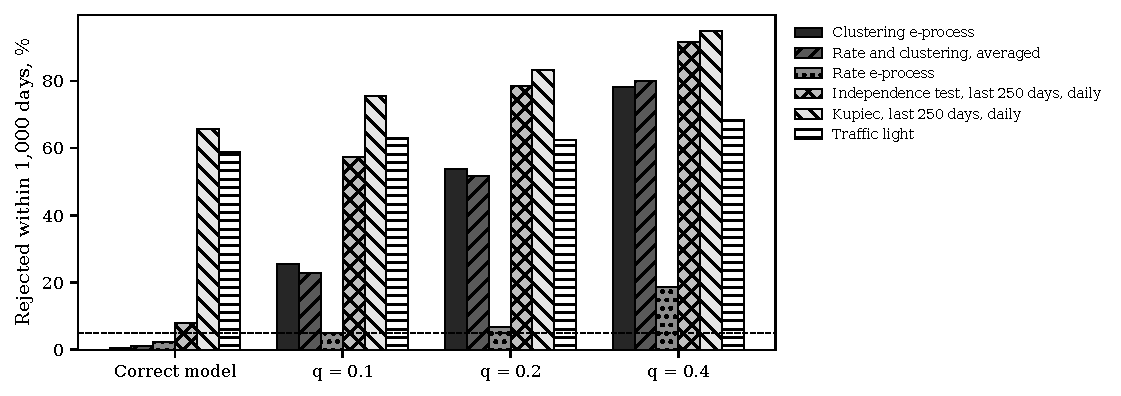
\includegraphics[width=0.9\textwidth]{clustering}
\caption{Share of streams of 1,000 days rejected at some day when the hit rate is right and a hit follows a hit with probability $q$, for the clustering and the rate e-processes, their average, the independence test and the Kupiec test on the last 250 days, the traffic light, each read every day, 2,000 streams per group; the first group is a correct model and the dashed line is 5\,\%.}
\label{fig:clustering}
\end{figure}

\subsection{Defaults against the PD of each grade}
\label{sec:results-pd}

\Cref{tab:pd-results} and \cref{fig:pd-books} (left) read the PD monitor on five grades over ten years. When the PD is right the product combination rejects \nPdOneProd\,\% and the average \nPdOneAvg\,\% of \nPdReps\ histories, while the chi-square test across grades read every year rejects \nPdOneChiEvery\,\%. When every PD is $1.1$ times the predicted one, the product rejects \nPdOneOneProd\,\%, the average \nPdOneOneAvg\,\% and the upper-side average \nPdOneOneAvgUp\,\% of the histories within ten years, while the chi-square test detects \nPdOneOneChiOne\,\% at year 10;
the median year of detection is \nPdMedYearOneOne\ for the upper-side average at that factor. At $1.05$ the monitors detect almost nothing (\nPdOneZeroFiveAvg\,\% for the average) against \nPdOneZeroFiveChiOne\,\% for the chi-square test at year 10. From $1.25$ every rule detects every history, the monitors at a median year of \nPdMedYearOneTwoFive. The size is held where the chi-square test read every year with its nominal critical value inflates it, but that is a property of the critical value and not of reading every year (a simulated critical value restores the size of the chi-square test and detects more, \cref{tab:pd-equal-size}), and the power cost for a small miscalibration is large: a ten-year cohort with a 5\,\% relative error in every grade is detected in \nPdOneZeroFiveChiOne\,\% of the histories by the chi-square test at year 10 and in \nPdOneZeroFiveAvgUp\,\% by the upper-side average e-process. The average detects more than the product at $1.1$ (\nPdOneOneAvg\ against \nPdOneOneProd\,\%), the reverse of what the independence assumed by the product would suggest;
\cref{sec:discussion} reads the difference through the growth-rate bound. When only the 10\,\% grade drifts (by $1.3$) every combination detects at least \nPdGradeProdUp\,\% of the histories (\cref{tab:ablation-pd}), so the average does not lose to the product where one grade carries the signal.

\begin{table*}[htbp]
\centering
\small
\caption{Defaults against the predicted PD of five grades (0.5 to 10\,\%), 2,000 obligors per grade and year, ten years, 1,000 histories per row from the generator of default counts: share of histories rejected at some year by the PD e-process combined by product or by average, by the chi-square test across grades on the cumulative counts read once at year 10, and by the same test read every year; the last column is the share of histories the upper-side average e-process rejects by year 3.}
\label{tab:pd-results}
\resizebox{\linewidth}{!}{%
\begin{tabular}{p{3.6cm}rrrrr}
\toprule
PD scaling & Product, \% & Average, \% & Chi-square at year 10, \% & Chi-square every year, \% & Average upper, by year 3, \% \\
\midrule
\relax 1 (size) & \relax 0.0 [0.0, 0.4] & \relax 0.4 [0.2, 1.0] & \relax 4.4 [3.3, 5.9] & \relax 20.8 [18.4, 23.4] & \relax 0.2 \\
\relax 1.05 & \relax 0.0 [0.0, 0.4] & \relax 2.9 [2.0, 4.1] & \relax 66.0 [63.0, 68.9] & \relax 78.7 [76.1, 81.1] & \relax 1.5 \\
\relax 1.1 & \relax 26.7 [24.1, 29.5] & \relax 55.9 [52.8, 58.9] & \relax 99.8 [99.3, 99.9] & \relax 99.8 [99.3, 99.9] & \relax 17.1 \\
\relax 1.25 & \relax 100.0 [99.6, 100.0] & \relax 100.0 [99.6, 100.0] & \relax 100.0 [99.6, 100.0] & \relax 100.0 [99.6, 100.0] & \relax 99.8 \\
\relax 10\% grade only, 1.3 & \relax 100.0 [99.6, 100.0] & \relax 100.0 [99.6, 100.0] & \relax 100.0 [99.6, 100.0] & \relax 100.0 [99.6, 100.0] & \relax 100.0 \\
\bottomrule
\end{tabular}}
\end{table*}


\Cref{tab:pd-correlation} and \cref{fig:pd-books} (right) show the effect \cref{prop:overdispersion} predicts. When the predicted PD is exactly right and the defaults of a year share a systematic factor, the two-sided e-processes reject \nRhoZeroThreeProd\,\% (product) and \nRhoZeroThreeAvg\,\% (average) of the histories at an asset correlation of $0.03$ and \nRhoOneTwoProd\ to \nRhoOneTwoAvg\,\% at $0.12$; the upper-side average rejects \nRhoZeroThreeAvgUp\,\% at $0.03$ and \nRhoTwoFourAvgUp\,\% at $0.24$. The chi-square test is not spared: it rejects \nRhoZeroThreeChiOne\,\% at year 10 and \nRhoZeroThreeChiEvery\,\% when read every year at $0.03$. At zero
correlation the sizes are those of \cref{tab:pd-results}. The loss is the loss of the binomial null that all these tests share, and the sequential construction inherits it and compounds it: the process grows by a factor above one in expectation at every year.

\begin{figure}[htbp]
\centering
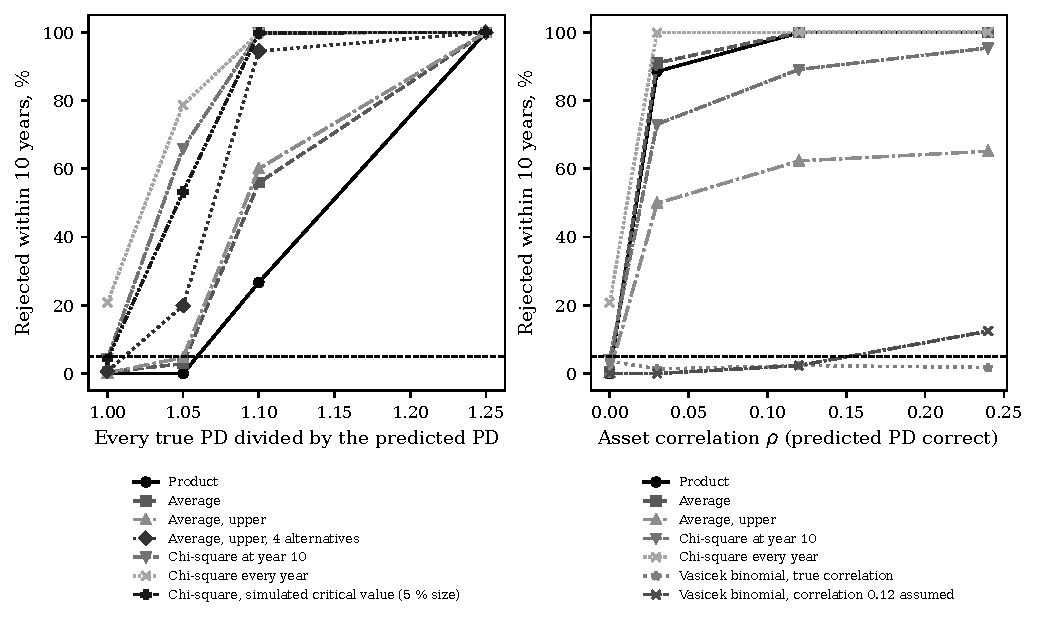
\includegraphics[width=\textwidth]{pd-books}
\caption{Share of ten-year histories of five rating grades rejected at some year. Left: every true PD is the predicted one multiplied by the factor on the horizontal axis, 1,000 histories per point, for the product and the average of the grade e-processes, the upper-side average with a coarse grid, and the chi-square test across grades. Right: the predicted PD is right and the defaults of each year share a systematic factor of asset correlation $\rho$, 2,000 histories per point, with the Vasicek-corrected binomial test of the engine at the true correlation and at an assumed correlation of 0.12; the dashed line is 5\,\%. The chi-square curve of the left panel uses a simulated critical value of size 5\,\%.}
\label{fig:pd-books}
\end{figure}

\begin{table*}[htbp]
\centering
\small
\caption{Share of 2,000 ten-year histories of five grades, with the predicted PD equal to the true PD, rejected at some year when the defaults of a year share one systematic factor of asset correlation $\rho$: the PD e-processes, whose null is binomial with no correlation, and the chi-square test across grades. The first row has no correlation and is the size under the null of both families.}
\label{tab:pd-correlation}
\resizebox{\linewidth}{!}{%
\begin{tabular}{rrrrrr}
\toprule
Asset correlation $\rho$ & Product, \% & Average, \% & Average, upper, \% & Chi-square at year 10, \% & Chi-square every year, \% \\
\midrule
\relax 0.00 & \relax 0.0 [0.0, 0.2] & \relax 0.6 [0.3, 1.0] & \relax 0.2 [0.1, 0.6] & \relax 4.2 [3.4, 5.1] & \relax 20.8 [19.0, 22.6] \\
\relax 0.03 & \relax 88.5 [87.0, 89.8] & \relax 91.0 [89.7, 92.2] & \relax 49.9 [47.7, 52.0] & \relax 73.0 [71.1, 74.9] & \relax 99.9 [99.6, 100.0] \\
\relax 0.12 & \relax 99.9 [99.6, 99.9] & \relax 100.0 [99.7, 100.0] & \relax 62.3 [60.2, 64.4] & \relax 89.1 [87.7, 90.4] & \relax 100.0 [99.8, 100.0] \\
\relax 0.24 & \relax 100.0 [99.8, 100.0] & \relax 100.0 [99.8, 100.0] & \relax 65.1 [63.0, 67.2] & \relax 95.4 [94.4, 96.2] & \relax 100.0 [99.8, 100.0] \\
\bottomrule
\end{tabular}}
\end{table*}


\Cref{tab:pd-comparators} runs the PD tests of the engine on the same histories. The exact binomial and the Jeffreys tests of each grade, read every year with a Bonferroni split, hold a size of \nPdcZeroBinEvery\ and \nPdcZeroJefEvery\,\% without correlation and reject \nPdcZeroThreeBinEvery\ and \nPdcZeroThreeJefEvery\,\% of the histories at an asset correlation of $0.03$, so they share the failure of the e-processes. The binomial test under the Vasicek one-factor mixture, which the engine carries as the remedy for correlated defaults, keeps its size when it is given the correlation that generated the histories: \nPdcZeroThreeVasTrueEvery\,\% at $0.03$, \nPdcOneTwoVasTrueEvery\,\% at $0.12$ and \nPdcTwoFourVasTrueEvery\,\% at $0.24$ (read once at year 10, \nPdcZeroThreeVasTrueOnce, \nPdcOneTwoVasTrueOnce\ and \nPdcTwoFourVasTrueOnce\,\%). With a correlation of \nPdcAssumedRho\ assumed it never rejects below that correlation (\nPdcZeroThreeVasAssumedEvery\,\% at $0.03$) and loses its size where the assumption is too low: \nPdcTwoFourVasAssumedEvery\,\% at $0.24$ (\nPdcTwoFourVasAssumedOnce\,\% read once). A comparator that holds its size under correlated defaults therefore exists, and the loss of size of the e-processes is not a consequence of reading every year; it is the consequence of a null without a correlation. The Vasicek test reads one year at a time and so does not pool the years as the e-process does; whether a monitor built on the same mixture would keep both the size and the pooling is the open step of \cref{sec:conclusions}.

\begin{table*}[htbp]
\centering
\small
\caption{The PD e-process and the PD tests of the engine on the same 2,000 histories as \cref{tab:pd-correlation} (predicted PD equal to the true PD, defaults of a year sharing a systematic factor of asset correlation $\rho$): share of histories rejected at some year, in percent with 95\,\% Wilson intervals. The per-grade tests (the exact binomial test, the Jeffreys test, and the binomial test under the Vasicek one-factor mixture with the correlation assumed or the true one) are one-sided; read every year they reject when any of the 5 grades in any of the 10 years has a p-value below $0.001$ (a Bonferroni split of 5\,\% over the 50 grade-years), and read once when any grade at year 10 is below $0.01$. The chi-square rule reads the statistic across grades every year against one critical value set by simulation on 50,000 correct histories to a size of 5\,\% over the ten years.}
\label{tab:pd-comparators}
\resizebox{\linewidth}{!}{%
\begin{tabular}{p{0.8cm}>{\raggedleft\arraybackslash}p{1.9cm}>{\raggedleft\arraybackslash}p{1.9cm}>{\raggedleft\arraybackslash}p{1.9cm}>{\raggedleft\arraybackslash}p{1.9cm}>{\raggedleft\arraybackslash}p{1.9cm}>{\raggedleft\arraybackslash}p{1.9cm}>{\raggedleft\arraybackslash}p{1.9cm}}
\toprule
$\rho$ & Average e-process & Binomial per grade & Jeffreys per grade & Vasicek, $0.12$ assumed & Vasicek, true $\rho$ & Vasicek, true $\rho$, read once & Chi-square, simulated critical value \\
\midrule
\relax 0.00 & \relax 0.6 [0.3, 1.0] & \relax 3.6 [2.9, 4.6] & \relax 4.1 [3.3, 5.1] & \relax 0.0 [0.0, 0.2] & \relax 3.6 [2.9, 4.6] & \relax 3.5 [2.7, 4.3] & \relax 4.4 [3.6, 5.4] \\
\relax 0.03 & \relax 91.0 [89.7, 92.2] & \relax 95.0 [94.0, 95.9] & \relax 95.3 [94.3, 96.1] & \relax 0.0 [0.0, 0.2] & \relax 1.4 [0.9, 2.0] & \relax 1.7 [1.2, 2.4] & \relax 99.2 [98.7, 99.5] \\
\relax 0.12 & \relax 100.0 [99.7, 100.0] & \relax 96.7 [95.8, 97.4] & \relax 96.8 [95.9, 97.4] & \relax 2.4 [1.8, 3.1] & \relax 2.4 [1.8, 3.1] & \relax 1.5 [1.1, 2.1] & \relax 100.0 [99.8, 100.0] \\
\relax 0.24 & \relax 100.0 [99.8, 100.0] & \relax 96.6 [95.7, 97.3] & \relax 96.7 [95.8, 97.4] & \relax 12.4 [11.1, 14.0] & \relax 1.8 [1.3, 2.4] & \relax 1.6 [1.1, 2.2] & \relax 100.0 [99.8, 100.0] \\
\bottomrule
\end{tabular}}
\end{table*}


The question the study asks of the PD monitor, whether the defaults of five grades are detected earlier than by the chi-square test read every year at an equal size, is answered by \cref{tab:pd-equal-size}. The chi-square test across grades is read every year against one constant critical value set by simulation on \nPdcCalReps\ correct histories, once to a size of 5\,\% over the ten years (a size of \nPdcOneChiSim\,\% on the histories of the table) and once to the size the average e-process measured, \nPdcMatchedSize\,\%. For a PD that is $5\,\%$ too low it rejects \nPdcOneZeroFiveChiSim\,\% of the histories within ten years (a median year of \nPdcOneZeroFiveChiSimYear) at the size of 5\,\% and \nPdcOneZeroFiveChiMatched\,\% at the size of the e-process, where the average e-process rejects \nPdOneZeroFiveAvg\,\%. For a PD that is $10\,\%$ too low the two chi-square rules reject \nPdcOneOneChiSim\,\% and \nPdcOneOneChiMatched\,\%, and \nPdcOneOneChiSimBy\ and \nPdcOneOneChiMatchedBy\,\% by year 3, against \nPdOneOneAvg\,\% and \nPdcOneOneAvgBy\,\% for the average e-process. From $1.25$ every rule rejects every history, the e-process at a median year of \nPdcOneTwoFiveAvgYear\ and the chi-square rules at \nPdcOneTwoFiveChiSimYear. At an equal size the defaults of the five grades are therefore not detected earlier by the e-process: on binomial defaults the chi-square rule detects a small miscalibration more often and sooner, and the e-process keeps what a simulated critical value lacks, a guarantee that does not depend on the horizon. The engine's per-grade binomial test, read every year with the Bonferroni split, detects \nPdcOneZeroFiveBinEvery\,\% at $1.05$ and \nPdcOneOneBinEvery\,\% at $1.1$.

\begin{table*}[htbp]
\centering
\small
\caption{Detection of a PD that is too low by the average PD e-process and by the chi-square test across grades read every year with a simulated constant critical value, at a size of 5\,\% and at the size the average e-process measured (0.4\,\%), on 1,000 histories per row (the histories of \cref{tab:pd-results}, no asset correlation). The first three rule columns give three numbers separated by slashes: the share of histories rejected within ten years (\%), the share rejected by year 3 (\%) and the median year of rejection among the histories rejected. The last two columns give the share rejected within ten years (\%) by the engine's binomial test per grade and by its Vasicek-corrected binomial test with a correlation of 0.12 assumed, each read every year with a Bonferroni split over the 50 grade-years.}
\label{tab:pd-equal-size}
\resizebox{\linewidth}{!}{%
\begin{tabular}{p{2.4cm}>{\raggedleft\arraybackslash}p{2.6cm}>{\raggedleft\arraybackslash}p{2.6cm}>{\raggedleft\arraybackslash}p{2.6cm}>{\raggedleft\arraybackslash}p{2.6cm}>{\raggedleft\arraybackslash}p{2.6cm}}
\toprule
PD scaling & Average e-process & Chi-square, 5\,\% size & Chi-square, size of the e-process & Binomial per grade, ever & Vasicek, $0.12$ assumed, ever \\
\midrule
\relax 1 (size) & \relax 0.4 / 0.4 / 1 & \relax 4.1 / 2.1 / 3 & \relax 0.4 / 0.2 / 4 & \relax 2.6 & \relax 0.0 \\
\relax 1.05 & \relax 2.9 / 0.8 / 4 & \relax 53.2 / 15.4 / 6 & \relax 23.2 / 2.4 / 7 & \relax 15.7 & \relax 0.0 \\
\relax 1.1 & \relax 55.9 / 13.8 / 6 & \relax 99.8 / 60.4 / 3 & \relax 98.8 / 29.3 / 5 & \relax 55.5 & \relax 0.0 \\
\relax 1.25 & \relax 100.0 / 99.7 / 2 & \relax 100.0 / 100.0 / 1 & \relax 100.0 / 100.0 / 1 & \relax 100.0 & \relax 0.0 \\
\relax 10\% grade only, 1.3 & \relax 100.0 / 100.0 / 1 & \relax 100.0 / 100.0 / 1 & \relax 100.0 / 100.0 / 1 & \relax 100.0 & \relax 0.0 \\
\bottomrule
\end{tabular}}
\end{table*}


\subsection{Real exceedances}
\label{sec:results-c11}

\Cref{tab:c11} reads the 18 models of the market-risk case at the 99\,\% level in the six windows. In the equity crisis of 2007 to 2009 every rule flags every model; the e-process flags them at a median day of \nCElevenEquityNinetyEMed, the Kupiec test on all days so far at \nCElevenEquityNinetyKupCumMed, and the traffic light at \nCElevenEquityNinetyLightMed (its first possible day). In the 2008 foreign-exchange window the e-process flags \nCElevenFxNinetyEFlag\ models at a median day of \nCElevenFxNinetyEMed, the traffic light \nCElevenFxNinetyLightFlag\ at day \nCElevenFxNinetyLightMed,
and the Kupiec test once at the end of the window \nCElevenFxNinetyKupEndFlag. Among the models the traffic light flags, the e-process misses \nCElevenFxNinetyLightMissedByE\ and flags the rest at a median day of \nCElevenFxNinetyLightE; it flags \nCElevenFxNinetyEOnlyVsKupiecEnd\ models that the end-of-window Kupiec test does not. In the window of 2020, with 104 days, the e-process flags \nCElevenCovidNinetyEFlag\ models at a median day of \nCElevenCovidNinetyEMed, and the traffic light cannot read the window at all; in 2022 (249 days), \nCElevenRatesNinetyEFlag\ at a median day of \nCElevenRatesNinetyEMed. In the 64 days of 2023 no rule flags any model.

\begin{table*}[htbp]
\centering
\small
\caption{The 18 models of the case on market risk in each of its six windows at the 99\,\% level: the number of models each rule flags at some day, and the median first-flag day among the models it flags. The rules are the rate e-process, the e-backtest of Wang, Wang and Ziegel (2022), the Kupiec test once at the end of the window (the eligibility gate), the Kupiec test on all days so far read daily from day 50, and the Basel traffic light, which needs 250 days (a dash where the window is shorter or the level is not the 99\,\% one). No truth is known in these windows.}
\label{tab:c11}
\resizebox{\linewidth}{!}{%
\begin{tabular}{lrrrrrrrrrr}
\toprule
Window & Days & Expected exceptions & E-process flags & Median day & E-backtest flags & Kupiec at end flags & Kupiec daily flags & Median day & Traffic light flags & Median day \\
\midrule
\relax calm-2004-06 & 750 & 7.5 & 2 & 352 & 1 & 3 & 7 & 70 & 9 & 252 \\
\relax equity-2007-09 & 504 & 5.0 & 18 & 24 & 18 & 18 & 18 & 50 & 18 & 250 \\
\relax fx-2008 & 251 & 2.5 & 9 & 68 & 7 & 7 & 18 & 68 & 11 & 250 \\
\relax equity-2020 & 104 & 1.0 & 12 & 25 & 6 & 13 & 13 & 50 & -- & -- \\
\relax rates-2022 & 249 & 2.5 & 8 & 52 & 3 & 8 & 17 & 54 & -- & -- \\
\relax mixed-2023 & 64 & 0.6 & 0 & -- & 0 & 0 & 0 & -- & -- & -- \\
\bottomrule
\end{tabular}}
\end{table*}


The calm window of 2004 to 2006 is the control: a quiet market in which the models should not be rejected systematically. The e-process flags \nCElevenCalmNinetyEFlag\ of the 18 models, the Kupiec test once at the end of the 750 days \nCElevenCalmNinetyKupEndFlag, and the e-backtest \nCElevenCalmNinetyWwzFlag; the rules read every day flag more: the Kupiec test on all days so far \nCElevenCalmNinetyKupCumFlag, the traffic light \nCElevenCalmNinetyLightFlag\ and the Kupiec test on the last 250 days \nCElevenCalmNinetyKupTrailFlag\ models. The 750 days give each of those rules
about three chances of an independent window, and the surplus of flags over the one-shot test is the repeated-reading inflation of \cref{prop:repeated} on real series, with the expected count of exceptions at the level in each model.
\Cref{fig:c11-days} compares the first flag of the e-process with that of the Kupiec test on all days so far for each model. In the crisis windows almost every model is flagged earlier by the e-process than the end of the window, and the Kupiec test on all days so far flags at the first look, day 50, in many models; in the calm window the points are few.

\begin{figure}[htbp]
\centering
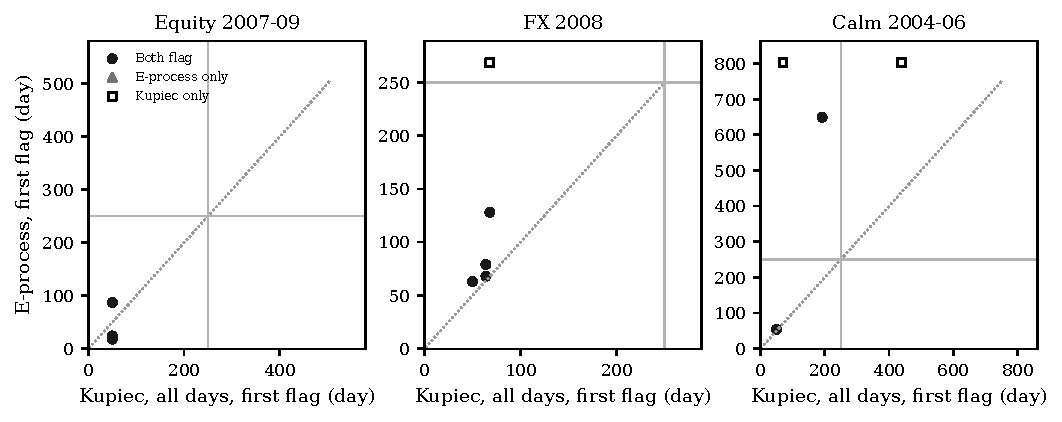
\includegraphics[width=\textwidth]{c11-days}
\caption{First day flagged by the rate e-process (vertical) against the first day flagged by the Kupiec test on all days so far (horizontal) for each of the 18 models at the 99\,\% level in three windows: the equity crisis, the foreign-exchange window of 2008 and the calm control window. Triangles on the right margin are models only the e-process flags and squares at the top are models only the Kupiec test flags; grey lines mark day 250.}
\label{fig:c11-days}
\end{figure}

At the 97.5\,\% level (\cref{tab:c11-975}) the e-process flags more models than the end-of-window Kupiec test in the windows of 2020 (\nCElevenCovidSeventyEFlag\ against \nCElevenCovidSeventyKupEndFlag), 2022 (\nCElevenRatesSeventyEFlag\ against \nCElevenRatesSeventyKupEndFlag) and 2008 (\nCElevenFxSeventyEFlag\ against \nCElevenFxSeventyKupEndFlag); in the calm window it flags fewer (\nCElevenCalmSeventyEFlag\ against \nCElevenCalmSeventyKupEndFlag). The comparison with the traffic light is
structurally in favour of the monitor, since the light cannot speak before day 250 and no rule of the set has a truth to be right against in these windows. The windows show when the rules fire, not which of them is right.

\begin{table*}[htbp]
\centering
\small
\caption{The 18 models of the case on market risk in each of its six windows at the 97.5\,\% level: the number of models each rule flags at some day, and the median first-flag day among the models it flags. The rules are the rate e-process, the e-backtest of Wang, Wang and Ziegel (2022), the Kupiec test once at the end of the window (the eligibility gate), the Kupiec test on all days so far read daily from day 50, and the Basel traffic light, which needs 250 days (a dash where the window is shorter or the level is not the 99\,\% one). No truth is known in these windows.}
\label{tab:c11-975}
\resizebox{\linewidth}{!}{%
\begin{tabular}{lrrrrrrrrrr}
\toprule
Window & Days & Expected exceptions & E-process flags & Median day & E-backtest flags & Kupiec at end flags & Kupiec daily flags & Median day & Traffic light flags & Median day \\
\midrule
\relax calm-2004-06 & 750 & 18.8 & 3 & 329 & 1 & 7 & 16 & 88 & -- & -- \\
\relax equity-2007-09 & 504 & 12.6 & 18 & 24 & 18 & 18 & 18 & 50 & -- & -- \\
\relax fx-2008 & 251 & 6.3 & 7 & 68 & 6 & 6 & 11 & 64 & -- & -- \\
\relax equity-2020 & 104 & 2.6 & 15 & 25 & 6 & 12 & 15 & 50 & -- & -- \\
\relax rates-2022 & 249 & 6.2 & 16 & 54 & 10 & 13 & 18 & 50 & -- & -- \\
\relax mixed-2023 & 64 & 1.6 & 0 & -- & 0 & 0 & 0 & -- & -- & -- \\
\bottomrule
\end{tabular}}
\end{table*}


\subsection{Real defaults by vintage}
\label{sec:results-c03}

\Cref{tab:c03} and \cref{fig:c03-paths} read the PD monitor on the five cohorts of small-business loans. The monitor looks for a vintage that defaults more than the predicted cumulative curve, with the vintages of a cohort as its grades and the ages as its steps, combined by average and by product. For the cohort of 2006 and 2007 and the cohort of 2008 to 2010 the monitor rejects at the first age, 12 months, with the largest value of $\log E$ of the average at \nCThreeMaxA\ and \nCThreeMaxB. The 2006 vintage has \nCThreeDTwoZeroZeroSix\ charge-offs against \nCThreePTwoZeroZeroSix\ predicted over the observed ages, the 2007 vintage \nCThreeDTwoZeroZeroSeven\ against \nCThreePTwoZeroZeroSeven. The binomial light read once at the five-year mark is red for these two vintages as well, 48 months later; the 2008 and 2009 vintages are red at the mark and rejected at 12 months, and the 2010 vintage is rejected at 24 months although its light is green and its charge-offs end below the predicted total (\nCThreeDTwoZeroOneZero\ against \nCThreePTwoZeroOneZero), a departure in the timing of the curve that a single reading at the mark does not see. No cohort from 2011 to 2020 is rejected as a cohort (the largest $\log E$ of an average is \nCThreeMaxE, below $\log 20=\nLogTwenty$): the model over-predicts, with for example \nCThreeDTwoZeroOneTwo\ charge-offs against \nCThreePTwoZeroOneTwo\ predicted in 2012, and a monitor of under-prediction has little to say. The 2018 vintage alone is rejected, at \nCThreeRejTwoZeroOneEight\ months ($\log E=\nCThreeVTwoZeroOneEight$), although its charge-offs end below the predicted total (\nCThreeDTwoZeroOneEight\ against \nCThreePTwoZeroOneEight); it is the same early-timing departure as the 2010 vintage, and the average over the three vintages of its cohort dilutes it. The values are the engine's output on the committed curves, recomputed here from the vintage curves with the product's builder and equal to the committed values for \nCThreeRebuilt\ of the five cohorts. Two to four vintages per cohort are few, and the binomial null has no asset correlation (\cref{prop:overdispersion}); the table illustrates the monitor on real curves and measures no power.

\begin{table*}[htbp]
\centering
\small
\caption{The PD e-process read at the ages 12, 24, 36, 48 and 60 months on the five cohorts of SBA 7(a) loans of the case on small-business credit, from the committed vintage curves: the charge-offs observed over the observed ages against the charge-offs the predicted curve implies, the first age at which each vintage and the cohort reject, and the light of the binomial test read once at the five-year mark. A dash means the monitor never reached 20.}
\label{tab:c03}
\resizebox{\linewidth}{!}{%
\begin{tabular}{llllllrr}
\toprule
Cohort & Vintages & Charge-offs / predicted & Month rejected, each & Five-year light, each & Month, average & Month, product & Largest $\log E$, average \\
\midrule
\relax FY2006-07 & \relax 2006, 2007 & \relax 19,271/7,601, 24,310/7,722 & \relax 12, 12 & \relax red, red & 12 & 12 & 11,631.0 \\
\relax FY2008-10 & \relax 2008, 2009, 2010 & \relax 13,088/4,526, 3,066/2,251, 1,954/2,158 & \relax 12, 12, 24 & \relax red, red, green & 12 & 12 & 6,362.5 \\
\relax FY2011-14 & \relax 2011, 2012, 2013, 2014 & \relax 1,662/2,957, 1,272/2,545, 1,240/2,506, 1,616/2,922 & \relax --, --, --, -- & \relax green, green, green, green & -- & -- & -2.5 \\
\relax FY2015-17 & \relax 2015, 2016, 2017 & \relax 2,134/4,886, 2,194/4,742, 2,417/4,508 & \relax --, --, -- & \relax green, green, green & -- & -- & -7.3 \\
\relax FY2018-20 & \relax 2018, 2019, 2020 & \relax 2,526/3,616, 1,786/2,630, 944/2,025 & \relax 12, --, -- & \relax green, green, green & -- & -- & 2.4 \\
\bottomrule
\end{tabular}}
\end{table*}


\begin{figure}[htbp]
\centering
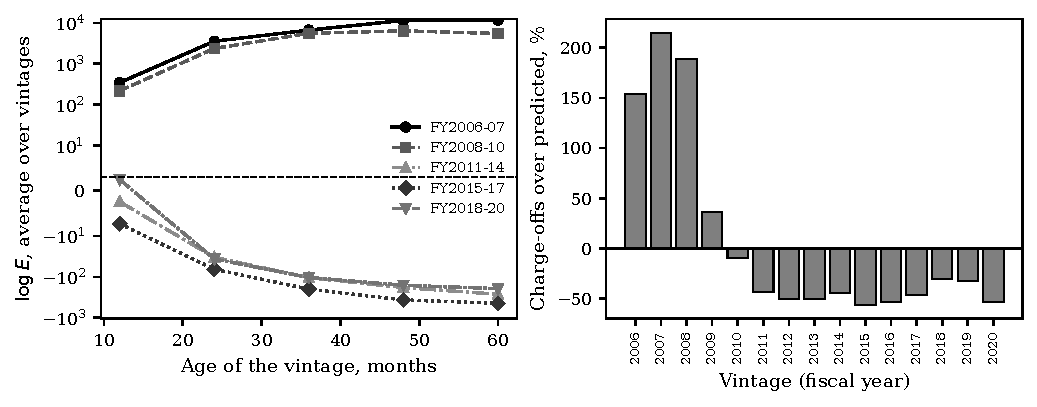
\includegraphics[width=\textwidth]{c03-paths}
\caption{Left: the log of the PD e-process averaged over the vintages of each cohort at the ages 12 to 60 months (symmetric logarithmic axis); the dashed line is the rejection threshold $\log 20$. Right: for each vintage, the charge-offs over the observed ages relative to the charge-offs of the predicted curve, in percent.}
\label{fig:c03-paths}
\end{figure}

\subsection{Agreement with the committed run and the outcome of the hypotheses}
\label{sec:results-agreement}

\Cref{tab:agreement} compares this study with the committed document of the product, which holds the same experiment from another seed. The shares ever rejected agree to within about one point (the Monte Carlo error of two runs of $2{,}000$ streams), and the median days agree to within the intervals of \cref{tab:main-results}, except the traffic light under clustering at $q=0.4$ (a median of \nCluMedFourTenthLight\ days in this run against \nCommittedCluMedFourTenthLight\ in the committed run); the committed medians at three and four times the nominal are \nCommittedMedThree\ and \nCommittedMedFour\ days, the power cost \nCommittedCostThree\ and \nCommittedCostFour\ points.
The committed document is also the product's own judgement of the hypotheses, and on one point this study reverses it. The document judges the delay hypothesis held at three times the nominal rate on one seed (a median of \nCommittedMedThree\ days against 250) and finds only the power cost failed (its verdict is that H3 failed and H1 and H2 held). On \nSeedsCount\ seeds the pooled median is \nSeedsThreeMed\ days (interval \nSeedsThreeMedLo\ to \nSeedsThreeMedHi), so that judgement of the delay does not survive replication; the spread of the median at three times the nominal in \cref{tab:x3-seeds} (a standard deviation of \nSeedsThreeSeedSd\ days between seeds) is of the size of the difference between the committed value and this run.

\begin{table*}[htbp]
\centering
\small
\caption{Agreement of this study with the committed document of the product (seed 42, 2,000 streams per scenario, same generator and engine release): the share of streams ever rejected and the median first-rejection day of three rules in four scenarios, the difference being the Monte Carlo error of two independent runs of 2,000 streams (about one point at the middle of the range).}
\label{tab:agreement}
\resizebox{\linewidth}{!}{%
\begin{tabular}{llrrrrr}
\toprule
Scenario & Rule & This run, ever, \% & Committed run, ever, \% & Difference, points & This run, median day & Committed run, median day \\
\midrule
\relax null & \relax Rate e-process & 2.4 & 1.8 & +0.6 & -- & -- \\
\relax null & \relax Kupiec, last 250 days & 65.7 & 66.5 & -0.8 & 718 & 704 \\
\relax null & \relax Traffic light & 58.8 & 58.7 & +0.1 & 812 & 840 \\
\relax rate x3 & \relax Rate e-process & 97.5 & 98.0 & -0.6 & 259 & 244 \\
\relax rate x3 & \relax Kupiec, last 250 days & 99.7 & 99.8 & -0.1 & 250 & 250 \\
\relax rate x3 & \relax Traffic light & 100.0 & 100.0 & +0.0 & 250 & 250 \\
\relax rate x4 & \relax Rate e-process & 100.0 & 100.0 & +0.0 & 130 & 129 \\
\relax rate x4 & \relax Kupiec, last 250 days & 100.0 & 100.0 & +0.0 & 250 & 250 \\
\relax rate x4 & \relax Traffic light & 100.0 & 100.0 & +0.0 & 250 & 250 \\
\relax cluster 0.4 & \relax Rate e-process & 18.6 & 18.2 & +0.4 & -- & -- \\
\relax cluster 0.4 & \relax Kupiec, last 250 days & 94.9 & 95.0 & -0.2 & 357 & 365 \\
\relax cluster 0.4 & \relax Traffic light & 68.3 & 66.8 & +1.5 & 622 & 670 \\
\bottomrule
\end{tabular}}
\end{table*}


\Cref{tab:hypotheses} gives the outcome of each hypothesis. H1 holds: the size is held and the repeated Kupiec rule exceeds it. H2 holds at four times the nominal and above and does not hold at three times for the two-sided monitor, whose pooled median is \nSeedsThreeMed\ days (interval \nSeedsThreeMedLo\ to \nSeedsThreeMedHi) against the 250 of the window and of the traffic light. H3 holds at four times the nominal and
fails at three times for the two-sided monitor (\nSeedsThreeCost\ points). The refutation clause, as the design states it on the equity and foreign-exchange windows, does not fire: the median day of the e-process among the models the traffic light flags is \nCElevenEquityNinetyLightE\ against \nCElevenEquityNinetyLightDay\ and \nCElevenFxNinetyLightE\ against \nCElevenFxNinetyLightDay. The same comparison on the generator, which this study adds to the clause, is the delay criterion of H2 and is reported there: at three times the nominal rate the pooled median, \nSeedsThreeMed, is not below the traffic light's \nSeedsThreeLight. The hypotheses as stated therefore do not hold as a whole: the delay and the power cost fail at three times the nominal rate and hold at four. The PD prediction is confirmed (\cref{sec:results-pd}). Two results were not pre-stated. The upper-side variant, which was chosen after the two-sided results, meets the delay and the power criteria at both severities on the same \nSeedsPooledN\ streams per factor; the choice is a finding that a prospective test would confirm, not a result of the pre-stated design. The PD question, whether the defaults of five grades are detected earlier than by the chi-square test at an equal size, was run after the other results and is answered no (\cref{sec:results-pd}).

\begin{table*}[htbp]
\centering
\small
\caption{The hypotheses of the proposed monitors, stated before the experiments, with the measurements that judge them and the outcome of each: size on the generator of known truth, delay and power cost pooled over 20 independent seeds of 2,000 streams, and the refutation clause on the generator and on the two real windows of the case on market risk at the 99\,\% level.}
\label{tab:hypotheses}
\resizebox{\linewidth}{!}{%
\begin{tabular}{p{6.0cm}p{6.6cm}p{2.4cm}}
\toprule
Hypothesis, stated before the experiments & Measured & Outcome \\
\midrule
\relax Size: the e-process rejects a correct VaR in at most $5\,\%$ plus three standard errors of the streams, read daily over 1,000 days, where the repeated Kupiec rule exceeds that & \relax e-process 2.4\,\%; Kupiec last 250 days 65.7\,\%, all days 31.9\,\%; bound 6.5\,\% & Held \\
\relax Delay: the median detection day is below the 250-day window, and below the traffic light's, at a hit rate three and four times too high & \relax x3: pooled median 251 [247, 255] (traffic light 250); 45\,\% of seeds below 250. x4: 128 [126, 129] (traffic light 250) & \relax x3: not met; x4: held \\
\relax Power cost: one Kupiec reading at day 250 has less than 10 points more power than the e-process has by day 250 & \relax x3: 12.4 $\pm$ 0.2 points; x4: 8.5 $\pm$ 0.2 points & \relax x3: not met; x4: held \\
\relax Upper-side variant of the rate monitor (chosen after the two-sided results, the direction a supervisor penalises): delay below 250 and below the traffic light's, and power cost under 10 points & \relax x3: pooled median 228 [225, 231], cost 6.7 $\pm$ 0.2 points; x4: 109 [108, 110], cost 4.6 $\pm$ 0.1 points & \relax Met at both severities \\
\relax Refutation clause: the hypothesis is refuted if the delay is not lower than the traffic light's, on the generator and on the equity 2007 to 2009 and foreign-exchange 2008 windows & \relax generator: x3 251 against 250, x4 128 against 250; real windows (models the light flags): median day 24 against 250 and 68 against 250 & \relax Fires at x3; not at x4 or on the real windows \\
\bottomrule
\end{tabular}}
\end{table*}

